\section{Degree-Corrected Stochastic Block Models}
\label{sec:ch5:dcsbm}


For this network model, we're going to start off with our school example that we covered in Section \ref{sec:ch5:sbm}. There are $100$ students, who each attend one of two schools. The edges of the network represent whether a pair of students are friends. If two students attend the same school, they have a higher chance of being friends than if they attend different schools. 

In a lot of real-world networks, this model works pretty effectively. It captures ``community structure'' in a very succinct way, but it has a glaring weakness. To explore this weakness, we would recommend that more advanced statistics users check out the Appendix Section \ref{sec:app:ch12:dcsbms}. Basically, the idea is this: within a given community, we have {no way} to represent fundamental differences between nodes in our SBM. Stated another way, if node $i$ and node $j$ are both in the same commuity, they will, on average, have the same {node degree}, which is a concept that you learned about in Section \ref{sec:ch4:prop-net:degree}. 

Rotating back to our school example from Section \ref{sec:ch5:sbm} to put this into context, on average, students in the network will have the same number of friends. This is referred to as the \textit{degree homogeneity} (the expected degrees are the same) for all nodes in the same community. Fortunately, there is a relatively easy way that we can rectify this issue and obtain a network model which does not suffer from this limitation: the degree-correction vector.

\subsection{The degree-correction vector allows us to convey node "importance"}

The reason that this equality in the number of expected ``friends'' for each student is problematic is that in real world networks, some nodes are more ``popular'' than others. This can be more generically conceptualized as some nodes being more ``important'' than others, in that they have a higher number of edges on average than other nodes in the network. This is known as \textit{degree heterogeneity}. The first two parameters of the DCSBM are the same as the SBM, in that we have a community assignment vector, and a block matrix.

The way that the degree heterogeneity is conveyed in a DCSBM is via the \textit{degree-correction vector} $\vec\theta$, which has $n$ elements (one for each node). For each node $i$, the degree-correction factor $\theta_i$ simply ``degree-corrects'' the node $i$, by either ``amplifying'' its expected node degree (meaning, on average, node $i$ will have {more} edges than it would if it were a node in a $SBM_n(\vec z, B)$) when $\theta_i > 1$, or ``reducing'' its expected node degree (meaning, on average, node $i$ will have {fewer} edges than it would if it were a node in a $SBM_n(\vec z, B)$) when $\theta_i < 1$. In general, degree correction factors are always taken to be $\geq 0$, which means that we cannot have a negative degree-correction factor. 

Rotating back to our coin flip example from Section \ref{sec:ch5:sbm}, let's conceptualize how we can break this down. For a given node pair of nodes $i$ and $j$, we look first at the community assignments of each of these nodes $z_{i}$ and $z_j$. Then, we take the corresponding entry from the block matrix, $b_{z_i z_j}$, which corresponds to the ``base'' probability that node $i$ and node $j$ are connected. Finally, we inflate (or deflate) this probability based on the degree-correction factors. We obtain a coin which lands on heads with probability $\theta_i \theta_j b_{z_iz_j}$, where $\theta_i$ and $\theta_j$ are the degree-correction factors for nodes $i$ and $j$. This gives us the probability of an edge $(i, j)$ existing between any given pair of nodes $i$ and $j$.

If $\mathbf A$ is a DCSBM random network with $n$ nodes, the community vector $\vec z$, the block matrix $B$, and the degree-correction factor $\vec\theta$, we say that $\mathbf A$ is a $DCSBM_n(\vec z, \vec \theta, B)$ random network. 

\subsection{Unifying $DCSBM_n(\vec z, \vec\theta, B)$ networks with the hierarchy of random network models}

As you might expect now that we have completed Section \ref{sec:ch5:ier} on IER random networks, the DCSBM can be easily tied to the IER random networks. Notice that above, we can take the probability $p_{ij} = \theta_i \theta_j b_{z_i z_j}$. This relationship demonstrates that there is a \textit{slight} condition on the vector $\vec \theta$ in order to ensure that the model that we specify is a valid random network model. In particular, for all pairs of nodes $i$ and $j$, the probability that an edge exists needs to be a probability, which means that it is between $0$ and $1$. 

To make this a little bit more concrete, a simple way to do this would be to develop a procedure for $P$ like we found for the SBM, and then check that $P$ is a matrix where all of its entries are between $0$ and $1$. To do this, we use the degree-correction matrix, which is simply a diagonal matrix whose entries are the degree-correction factors. We will denote this matrix with $n$ rows and $n$ columns by $\Theta$ (uppercase $\theta$, since it is a matrix):

\begin{align}
    \Theta &= \begin{bmatrix}
        \theta_1 & 0 & \cdots & 0 \\
        0 & \theta_2 & \ddots & \vdots \\
        \vdots & \ddots & \ddots & 0 \\
        0 & \cdots & 0 & \theta_n
    \end{bmatrix}.
    \label{eqn:ch5:dcsbm:Theta}
\end{align}

The procedure to generate a probability matrix for a $DCSBM_n(\vec z, \vec\theta, B)$ network is indicated in Algorithm \ref{alg:ch4:thresholding}. Basically, the idea is to just use the procedure to generate a probability matrix for an $SBM_n(\vec z, B)$ random network, and use this as the ``uncorrected probability matrix''. Then, simply apply the degree-correction, by pre-multiplying by $\Theta$ and $\Theta^\top$. 

\begin{algorithm}[h]\caption{Generating a probability matrix for a $DCSBM_n(\vec z, \vec\theta, B)$}
\label{alg:ch5:dcsbm_prob}
\SetAlgoLined
\KwData{$n$ a number of nodes\newline $\vec z$ a community-assignment vector of each node to one of $K$ communities \newline $\vec \theta$ a degree-correction factor\newline $B$ a block matrix with $K$ rows and $K$ columns}
\KwResult{A probability matrix for a $DCSBM_n(\vec z, \vec \theta, B)$.}

Let $P' = CBC^\top$, as-per Algorithm \ref{alg:ch5:sbm_pmtx}, where $C$ is the one-hot encoding of $\vec z$.

Let $\Theta$ be the degree-correction matrix, defined as-per Equation \ref{eqn:ch5:dcsbm:Theta}.

Let $P = \Theta P' \vec\Theta^\top$. 

\Return{$P$}
\end{algorithm}
From Section \ref{sec:ch5:ier:ier_generalises}, notice that $P'$ is the matrix where $p_{ij}' = b_{z_i z_j}$. It looks like this:
\begin{align*}
    P' &= \begin{bmatrix}
        b_{z_1 z_1} & \hdots & b_{z_1 z_n} \\
        \vdots  &\ddots & \vdots \\
        b_{z_n z_1} & \hdots & b_{z_n z_n}
    \end{bmatrix}.
\end{align*}
When we pre-multiply by $\Theta$, we get:
\begin{align*}
    \Theta P' &= \begin{bmatrix}
        \theta_1 b_{z_1z_1} & \hdots & \theta_1 b_{z_1 z_n} \\
        \vdots & \ddots & \vdots \\
        \theta_n b_{z_nz_1} & \hdots & \theta_n b_{z_n z_n}
    \end{bmatrix},
\end{align*}
and when we post-multiply this by $\Theta^\top$, we get:
\begin{align*}
    \Theta P' \Theta^\top &= \begin{bmatrix}
        \theta_1^2 b_{z_1z_1} & \hdots & \theta_1\theta_n b_{z_1 z_n} \\
        \vdots & \ddots & \vdots \\
        \theta_n \theta_1 b_{z_nz_1} & \hdots & \theta_n^2 b_{z_n z_n}
    \end{bmatrix}.
\end{align*}

This means that:
\begin{align*}
    p_{ij} = (\Theta P' \Theta^\top)_{ij} = \theta_i \theta_j b_{z_i z_j}.
\end{align*}

Notice that the entries of this matrix are exactly the probability of an edge existing in a $DCSBM_n(\vec z, \vec \theta, B)$ random network. In this sense, we can think of the degree-correction factor $\vec \theta$ as ``inflating'' or ``deflating'' the block probabilities of an $SBM_n(\vec z, B)$ random network based on a node's popularity $\theta_i$ or $\theta_j$. We can observe this by comparing the result that we obtained above with the result that we saw in Equation \eqref{eqn:ch5:ier:sbm_p}. We will pivot back to this observation in Section \ref{sec:ch5:psd_block:same_lp} to study it more in-depth.

\begin{floatingbox}[h]\caption{When is a degree-correction vector $\vec \theta$ valid?}
Technically, not every choice of a degree-correction vector will be valid, in that the equation $P = \Theta CBC^\top \Theta^\top$ that you described above might not {necessarily} produce a probability matrix. To ensure that it is a probability matrix, all that we need to do is ensure that $\vec\theta$ is a vector and $B$ is a probability matrix where the resulting $P$ matrix has entries which are between $0$ and $1$.

If you are using $DCSBM_n(\vec z, \vec \theta, B)$ for simulations or for toying around, one very easy way to do this is to just choose $\theta$ such that the maximum value is $1$, and then adjust $B$ accordingly. The product of a degree-correction factor (which is between $0$ and $1$) and a block probability (which is also between $0$ and $1$) will always be a probability (between $0$ and $1$), so either of these approaches are guaranteed to produce degree-correction factors that produce valid probability matrices.

 Another popular way to do this \cite{Karrer2011Jan,Qin2013Sep} would be to select $\vec \theta$ such that for every community, all of the degree-correction factors within that community sum to $1$. This means that the entries $\theta_i$ will be strictly less than $1$ if there are at least two nodes in a single community. This has the implication that the block matrix could be adjusted such that it is no longer a probability matrix, and you could still end up with a valid probability matrix using $P = \Theta C B C^\top \Theta^\top$. 
 
 We will tend to prefer the former for the purposes of this book, simply because it's easier to grasp at an introductory level, as it doesn't change any of the intuition that you've been building up from $SBM_n(\vec z, B)$ random networks (whereas, the latter will no longer have $B$ necessarily a block probability matrix). When doing complicated theoretical proofs with $DCSBM_n(\vec z, \vec\theta, B)$ random networks, the latter qualification tends to be easier to work with.
\end{floatingbox}

\subsubsection{When are $DCSBM_n(\vec z, \vec \theta, B)$ random networks $RDPG_n(X)$ random networks?}
\label{sec:ch5:dcsbm:rdpg}
As you can see in Algorithm \ref{alg:ch5:dcsbm_prob}, the probability matrix for a $DCSBM_n(\vec z, \vec \theta, B)$ random network is $P = \Theta P' \Theta^\top$, where $P'$ was the uncorrected probability matrix for an $SBM_n(\vec z, B)$ random network. Plugging in that $P' = CBC^\top$, we get that:
\begin{align*}
    P = \Theta C B C^\top \Theta^\top.
\end{align*}
As we concluded in Section \ref{sec:ch5:ier:rdpg_sbm}, we could produce a latent position matrix $X$ for any probability matrix which was positive semi-definite. As it turns out, the condition for the probability matrix $P$ of a $DCSBM_n(\vec z, \vec \theta, B)$ random network to be positive semi-definite is {identical} to that of an $SBM_n(\vec z, B)$ random network: the block matrix $B$ must be positive semi-definite. To recap, if the block matrix $B$ is positive semi-definite, it has a matrix $\sqrt B$ where $B = \sqrt B \sqrt B^\top$, so letting $X = \Theta C \sqrt B$, we can see that:
\begin{align*}
    XX^\top &= \Theta C \sqrt B \left (\Theta C \sqrt B\right )^\top \\
    &= \Theta C \sqrt B \sqrt B^\top C^\top \Theta^\top \\
    &= \Theta C B C^\top \Theta^\top,
\end{align*}
where in the last line we used the fact that $\sqrt B\sqrt B^\top = B$. 

This means that the $DCSBM_n(\vec z, \vec \theta, B)$ random networks with fewer communities than nodes which have a positive semi-definite probability matrix are less complex than the $RDPG_n(X)$ random networks. Further, the $DCSBM_n(\vec z, \vec \theta, B)$ random networks with fewer communities than nodes are more complex than the $SBM_n(\vec z, B)$ random networks with fewer communities than nodes, because we could always just take the degree-correction factor $\vec \theta$ to be a vector of ones for any possible community-assignment vector $\vec z$ and block matrix $B$. However, the reverse does not hold true. To think about this, try to imagine what happens when the degree-correction vector has a unique value for each node. Finally, the $DCSBM_n(\vec z, \vec \theta, B)$ random networks with indefinite probability matrices are distinct from $RDPG_n(X)$ random networks.

\subsection{How do you simulate samples of a $DCSBM_n(\vec z, \vec \theta, B)$ random network?}

While \texttt{graspologic} and \texttt{networkx} do not have utilities built-in to allow us to simulate samples of a DCSBM directly, we can use the tools we have just developed to write our own simulation ourselves. The procedure below will produce for you a network $A$, which has nodes and edges, where the underlying random network $\mathbf A$ is a DCSBM random network:

\begin{algorithm}[h]\caption{Simulating a sample from a $DCSBM_n(\vec z, \vec \theta, B)$ random network}
\label{alg:ch5:sbm}
\SetAlgoLined
\KwData{$n$ a number of nodes\newline $\vec z$ a community assignment vector of each of the $n$ nodes to $K$ communities \newline $\vec \theta$ a valid degree-correction vector for each of the $n$ nodes \newline $B$ a block matrix with $K$ rows and $K$ columns}
\KwResult{The adjacency matrix of a sample from the random network.}

Define $P = \Theta CBC^\top \Theta^\top$ as-per Algorithm \ref{alg:ch5:dcsbm_prob}, using $\vec z$, $\vec \theta$, and $B$, where $C$ is the one-hot encoding of $\vec z$, and $\Theta$ is the degree-correction matrix.

Generate a sample $A$ from an $IER_n(P)$ network.

\Return{$A$}
\end{algorithm}

Let's see how this works out in practice. In our example, we'll assume that students are ordered by their popularity, via a degree-correction vector that declines from $1$ to $0.5$ in the first community, and then has the same set of values for the second community. We'll borrow the \texttt{generate\_sbm\_pmtx()} utility from Section \ref{sec:ch5:ier:sbm_pmtx}:

\begin{lstlisting}[style=python]
import numpy as np
from graspologic.simulations import sample_edges
from graphbook_code import heatmap, plot_vector, \
    generate_sbm_pmtx

def dcsbm(z, theta, B, directed=False, loops=False, return_prob=False):
    """
    A function to sample a DCSBM.
    """
    # uncorrected probability matrix
    Pp = generate_sbm_pmtx(z, B)
    theta = theta.reshape(-1)
    # apply the degree correction
    Theta = np.diag(theta)
    P = Theta @ Pp @ Theta.transpose()
    robj = sample_edges(P, directed=directed, loops=loops)
    if return_prob:
        robj = (robj, P)
    return robj

nk = 50  # 50 students per school
z = np.array([1 for i in range(nk)] + [2 for i in range(nk)])
B = np.array([[0.6, 0.2], [0.2, 0.4]])  # same probabilities as from SBM section
theta = np.tile(np.linspace(1, 0.5, nk), 2)
A, P = dcsbm(z, theta, B, return_prob=True)
plot_vector(z, title="$\\vec z$", legend_title="School", color="qualitative", 
            ticks=[0.5, 49.5, 99.5], ticklabels=[1, 50, 100],
            ticktitle="Student")
plot_vector(theta, title="$\\vec \\theta$", 
            legend_title="Degree-Correction Factor", 
            ticks=[0.5, 49.5, 99.5], ticklabels=[1, 50, 100],
            ticktitle="Student")
heatmap(P, title="$P = \\Theta C B C^\\top \\Theta^\\top$")
heatmap(A.astype(int), title="Sample of $DCSBM_n(\\vec z, \\vec \\theta, B)$")
\end{lstlisting}
We can visualize the parameters for the $DCSBM_n(\vec z, \vec \theta, B)$ random network that we sampled in Figure \ref{fig:ch5:dcsbm}. Notice in particular that the degree-correction factors in Figure \ref{fig:ch5:dcsbm}(B) are higher for the first nodes in each community. This is reflected in the probability matrix in Figure \ref{fig:ch5:dcsbm}(D), where the probabilities are highest in the upper-left corners (which consist of edges between nodes with high degree-correction factors). In this sense, any edges between a pair of nodes with high degree-correction factors will tend to have a higher probability of existing than edges between pairs of nodes with lower degree-correction factors.

\begin{figure}[h]
    \centering
    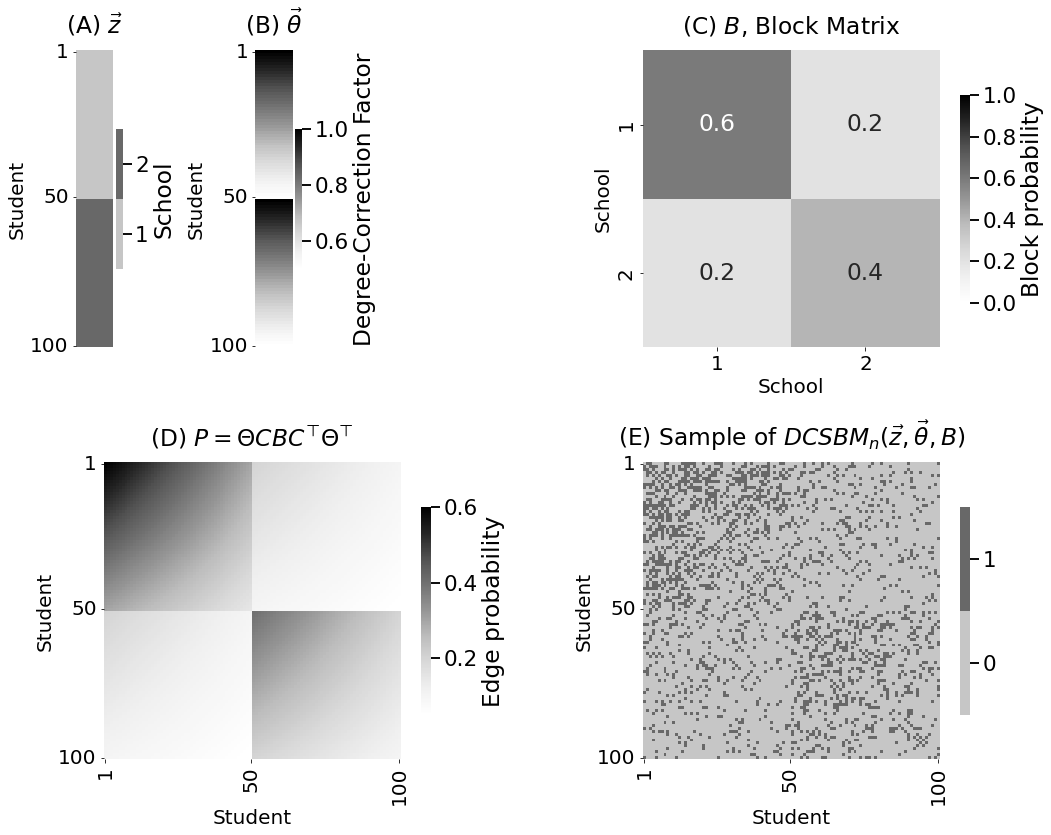
\includegraphics[width=0.9\linewidth]{representations/ch5/Images/dcsbm.png}
    \caption[Parameters of $DCSBM_n(\vec z, \vec \theta, B)$ random network]{\textbf{(A)} the community assignment vector, \textbf{(B)} the degree-correction vector, and \textbf{(C)} the block probability matrix. \textbf{(D)} the probability matrix, calculated from the community assignment vector, the degree-correction vector, and the degree-correction factor. \textbf{(E)} a sample from a $DCSBM_n(\vec z, \vec \theta, B)$ random network, using the probability matrix from \textbf{(D)} coupled with an $IER_n(P)$ network sampler from \texttt{graspologic}.}
    \label{fig:ch5:dcsbm}
\end{figure}

\subsection{Why is it called a degree-corrected stochastic block model?}

To begin to understand this, we will first think about the stochastic block model. Let's imagine that $\mathbf A$ is a $SBM_n(\vec z, B)$ random network with two communities. Let's imagine that the node $i$ is in community $1$, so $z_i = 1$. The expected node degree for a node $i$ in community $1$ can be written:
\begin{align*}
    \mathbb E[\mathbf d_i ; z_i = 1] &= \sum_{j \neq i} \mathbb E[\mathbf a_{ij}; z_i = 1] = \sum_{j \neq i}p_{ij}.
\end{align*}
All that the semicolon means is that we are proceeding with the assumption that we are calculating the expected degree for a node where $z_i = 1$ (the node $i$ is in communuity $1$). 

For the stochastic block model, this relationship is extremely simple. If node $i$ is in community $1$, this sum can be split into:
\begin{align*}
    \mathbb E[\mathbf d_i ; z_i = 1] &= \sum_{j : z_j = 2}p_{ij} + \sum_{j : z_j = 1\text{ and }j \neq i}p_{ij},
\end{align*}
So basically, we have split the sum into a sum over the other nodes in community $2$ (where $z_j = 2$) and the nodes that are not node $i$ but are also in community $1$. Note that for nodes in community $2$, $p_{ij} = b_{12}$. For nodes in community $1$, $p_{ij} = b_{11}$. Therefore:
\begin{align*}
    \mathbb E[\mathbf d_i ; z_i = 1] &= n_2 b_{12} + (n_1 - 1) b_{11}.
\end{align*}
Notice that nothing in the result here depends on the node, other than its community assignment. This means that for a $SBM_n(\vec z, B)$ random network, the nodes all have the same expected degree (if they are in the same community). This is known as the \textit{degree-homogeneity within-community} of the stochastic block model: all nodes (in the same community) have the same node expected node degree.

On the other hand, let's imagine that the network is a $DCSBM_n(\vec z, \vec \theta, B)$ random network. This expression gets a little more complicated, and becomes:
\begin{align*}
    \mathbb E[\mathbf d_i ; z_i = 1] &= \sum_{j \neq i} \mathbb E[\mathbf a_{ij}] = \sum_{j \neq i}\theta_i\theta_j p_{ij}.
\end{align*}
When we work through the same math as we showed above, this time we get:
\begin{align*}
    \mathbb E[\mathbf d_i ; z_i = 1] &= \theta_i \left(n_2 b_{12}\sum_{j : z_j = 2}\theta_j + (n_1 - 1) b_{11}\sum_{j : z_j = 1\text{ and }j \neq i}\theta_j\right),
\end{align*}
and the expected degree of the node $i$ is ``degree-corrected'' by its degree-correction factor $\theta_i$. 

\begin{floatingbox}[h]\caption{The expected node degree for block models}
If $\mathbf A$ is a $SBM_n(\vec z, B)$ random network with $n$ nodes and $K$ communities, then the expected degree of a node $i$ is:
\begin{align*}
    \mathbb E[\mathbf d_i ; z_i = k] &= \sum_{l \neq k} n_l b_{lk} + (n_k - 1)b_{kk}.
\end{align*}
If $\mathbf A$ is a $DCSBM_n(\vec z, \vec \theta, B)$ random network with $n$ nodes and $K$ communities, then the expected degree of a node $i$ is:
\begin{align*}
    \mathbb E[\mathbf d_i; z_i = k] &= \theta_i \left(\sum_{l \neq k}\left[n_l b_{lk}\sum_{j : z_j = l}\theta_j\right] + (n_k - 1)b_{kk}\sum_{j : z_j = k\text{ and }j \neq i}\theta_j\right).
\end{align*}
\end{floatingbox}

\newpage